\documentclass{assignment}
\usepackage[pdftex]{graphicx}
\usepackage{xcolor}
\definecolor{LightGray}{gray}{0.95}
\usepackage{fancyvrb, minted}
\usepackage[letterpaper, margin = 2.5cm]{geometry}
\usepackage[T1]{fontenc}
\usepackage{amsmath, amsfonts, amssymb}
\usepackage{hyperref, url} 
\usepackage{fancyhdr}
\usepackage{enumitem}
\usepackage{listings}

\newcommand{\R}{\mathbb{R}}

\student{Aren Ashlock}   
\semester{Spring 2024}                         
\date{February 29, 2024}  

\courselabel{COM S 474/574} 
\exercisesheet{HW3}{Optimization}

\school{Department of Computer Science}
\university{Iowa State University}

\begin{document}
\begin{problem}

%----------------------------------------- 1 DONE -----------------------------------------

\section{Definitions}

\begin{enumerate}

    \item Are the following sets convex?
    
    \begin{enumerate}[label=(\alph*)]

%---------------------------------------- 1A DONE -----------------------------------------
    
        \item $\{x | x \in \R^2, x^Tx \leq 2\}$

        \color{blue}\textbf{Answer:} IS convex\color{black}

%------------------------------------------------------------------------------------------

%---------------------------------------- 1B DONE -----------------------------------------
        
        \item $\{x | x \in \R^2, x^Tx \geq 2\}$

        \color{blue}\textbf{Answer:} IS convex\color{black}

%------------------------------------------------------------------------------------------

    \end{enumerate}

%----------------------------------------- 2 DONE -----------------------------------------
        
    \item Are the following sets strictly convex?

    \begin{enumerate}[label=(\alph*)]

%------------------------------------------------------------------------------------------

%---------------------------------------- 2A DONE -----------------------------------------
        
        \item $\{x | x \in \R^2, x^Tx \leq 2\}$

        \color{blue}\textbf{Answer:} IS strictly convex\color{black}

%------------------------------------------------------------------------------------------

%---------------------------------------- 2B DONE -----------------------------------------

        \item $\{x | Ax \leq 0\}$ ($A = \begin{bmatrix}
            1 & 1\\
            1 & -1
        \end{bmatrix}$)

        \color{blue}\textbf{Answer:} IS NOT strictly convex\color{black}

%------------------------------------------------------------------------------------------

    \end{enumerate}

%----------------------------------------- 3 DONE -----------------------------------------
        
    \item Are the following functions convex?

    \begin{enumerate}[label=(\alph*)]

%------------------------------------------------------------------------------------------

%---------------------------------------- 3A DONE -----------------------------------------
        
        \item $f(x) = x^2, x \in \R$

        \color{blue}\textbf{Answer:} IS convex\color{black}

%------------------------------------------------------------------------------------------

%---------------------------------------- 3B DONE -----------------------------------------
        
        \item $f(x) = x^2, x \in [0,1]$

        \color{blue}\textbf{Answer:} IS convex\color{black}

%------------------------------------------------------------------------------------------

%---------------------------------------- 3C DONE -----------------------------------------
        
        \item $f(x) = x^Tx + 4, x \in \R^2$

        \color{blue}\textbf{Answer:} IS convex\color{black}

%------------------------------------------------------------------------------------------

%---------------------------------------- 3D DONE -----------------------------------------

        \item $f(x) = x^Tx + 4, x \in \R^2, x^Tx \geq 2$

        \color{blue}\textbf{Answer:} IS convex\color{black}

%------------------------------------------------------------------------------------------

    \end{enumerate}

%----------------------------------------- 4 DONE -----------------------------------------
        
    \item Are the following matrices Positive Definite (PD), Positive Semi-Definite (PSD), Negative Definite (ND), or Negative Semi-Definite (NSD)? Please explain your answers.

    \begin{enumerate}[label=(\alph*)]

%------------------------------------------------------------------------------------------

%---------------------------------------- 4A DONE -----------------------------------------
        
        \item $\begin{bmatrix}
            0 & 0\\
            0 & 4
        \end{bmatrix}$

        \color{blue}\textbf{Answer:} PSD
        
        $det(\begin{bmatrix}
            0 - \lambda & 0 \\
            0 & 4 - \lambda
        \end{bmatrix}) = 0 \rightarrow \lambda = 4, 0 \rightarrow \lambda_i \geq 0, \forall i$\color{black}

%------------------------------------------------------------------------------------------

%---------------------------------------- 4B DONE -----------------------------------------
        
        \item $\begin{bmatrix}
            1 & 1\\
            1 & 4
        \end{bmatrix}$

        \color{blue}\textbf{Answer:} PD
        
        $det(\begin{bmatrix}
            1 - \lambda & 1 \\
            1 & 4 - \lambda
        \end{bmatrix}) = 0 \rightarrow \lambda \approx 4.3, 0.7 \rightarrow \lambda_i > 0, \forall i$\color{black}

%------------------------------------------------------------------------------------------

%---------------------------------------- 4C DONE -----------------------------------------
        
        \item $\begin{bmatrix}
            -5 & 2 & 0\\
            2 & -3 & 1\\
            0 & 1 & -2
        \end{bmatrix}$

        \color{blue}\textbf{Answer:} ND
        
        $det(\begin{bmatrix}
            -5 - \lambda & 2 & 0 \\
            2 & -3 - \lambda & 1 \\
            0 & 1 & -2 - \lambda
        \end{bmatrix}) = 0 \rightarrow \lambda \approx -6.3, -2.7, -1 \rightarrow \lambda_i < 0, \forall i$\color{black}

%------------------------------------------------------------------------------------------

    \end{enumerate}

%----------------------------------------- 5 DONE -----------------------------------------
        
    \item Are the following functions Lipschitz continuous? Why?

    \begin{enumerate}[label=(\alph*)]

%------------------------------------------------------------------------------------------

%---------------------------------------- 5A DONE -----------------------------------------
        
        \item $f(x) = \sqrt{x}, x \in [0,1]$

        \color{blue}\textbf{Answer:} IS NOT Lipschitz continuous $\rightarrow ||\sqrt{x}|| = \frac{1}{2\sqrt{x}}$, which cannot be bounded by L for all x \color{black}

%------------------------------------------------------------------------------------------

%---------------------------------------- 5B DONE -----------------------------------------
        
        \item $f(x) = x^2, x \in \R$

        \color{blue}\textbf{Answer:} IS NOT Lipschitz continuous $\rightarrow ||x^2|| = 2x$, which cannot be bounded by L for all x \color{black}

%------------------------------------------------------------------------------------------

%---------------------------------------- 5C DONE -----------------------------------------
        
        \item $f(x) = x^2, x \in [0,1]$

        \color{blue}\textbf{Answer:} IS Lipschitz continuous $\rightarrow ||x^2|| = 2x$, which $\forall x, 2x \leq 2$, so it is bounded when $L \geq 2$ \color{black}

%------------------------------------------------------------------------------------------

%---------------------------------------- 5D DONE -----------------------------------------

        \item $f(x) = |x|, x \in \R$

        \color{blue}\textbf{Answer:} IS Lipschitz continuous $\rightarrow ||(|x|)|| = \frac{x}{|x|}$, which $\forall x, \frac{x}{|x|} \leq 1$, so it is bounded when $L \geq 1$\color{black}

%------------------------------------------------------------------------------------------

%---------------------------------------- 5E DONE -----------------------------------------
        
        \item $f(x) = \sqrt{7x^2 + 4}, x \in \R$

        \color{blue}\textbf{Answer:} IS Lipschitz continuous $\rightarrow ||\sqrt{7x^2 + 4}|| = \frac{7x}{\sqrt{7x^2 + 4}}$, which $\forall x, \frac{7x}{\sqrt{7x^2 + 4}} \leq \sqrt{7}$, so it is bounded when $L \geq \sqrt{7}$ \color{black}

%------------------------------------------------------------------------------------------

%---------------------------------------- 5F DONE -----------------------------------------
        
        \item $f(x) = \text{sin } x, x \in \R$

        \color{blue}\textbf{Answer:} IS Lipschitz continuous $\rightarrow ||\text{sin } x|| = \text{cos } x$, which $\forall x, \text{cos } x \leq 1$, so it is bounded when $L \geq 1$ \color{black}

%------------------------------------------------------------------------------------------

%---------------------------------------- 5G DONE -----------------------------------------
        
        \item $f(x) = x^5, x \in \R$

        \color{blue}\textbf{Answer:} IS NOT Lipschitz continuous $\rightarrow ||x^5|| = 5x^4$, which cannot be bounded by L for all x \color{black}

%------------------------------------------------------------------------------------------

    \end{enumerate}

%----------------------------------------- 6 DONE -----------------------------------------
        
    \item Are the following functions Lipschitz smooth? Why?

    \begin{enumerate}[label=(\alph*)]

%------------------------------------------------------------------------------------------

%---------------------------------------- 6A DONE -----------------------------------------
        
        \item $f(x) = \sqrt{x}, x \in [0,1]$

        \color{blue}\textbf{Answer:} IS NOT Lipschitz smooth $\rightarrow H(\sqrt{x}) = \frac{-1}{4x^{3/2}}$, which cannot be bounded by L for all x \color{black}

%------------------------------------------------------------------------------------------

%---------------------------------------- 6B DONE -----------------------------------------
        
        \item $f(x) = x^2, x \in \R$

        \color{blue}\textbf{Answer:} IS Lipschitz smooth $\rightarrow H(x^2) = 2$, which $\forall x, 2 \leq 2$, so it is bounded when $L \geq 2$ \color{black}

%------------------------------------------------------------------------------------------

%---------------------------------------- 6C DONE -----------------------------------------
        
        \item $f(x) = x^2, x \in [0,1]$

        \color{blue}\textbf{Answer:} IS Lipschitz smooth $\rightarrow H(x^2) = 2$, which $\forall x, 2 \leq 2$, so it is bounded when $L \geq 2$ \color{black}

%------------------------------------------------------------------------------------------

%---------------------------------------- 6D DONE -----------------------------------------

        \item $f(x) = |x|, x \in \R$

        \color{blue}\textbf{Answer:} IS NOT Lipschitz smooth since $|x|$ is not twice differentiable \color{black}

%------------------------------------------------------------------------------------------

%---------------------------------------- 6E DONE -----------------------------------------
        
        \item $f(x) = \sqrt{7x^2 + 4}, x \in \R$

        \color{blue}\textbf{Answer:} IS Lipschitz smooth $\rightarrow H(\sqrt{7x^2 + 4}) = \frac{28}{(7x^2 + 4)^{3/2}}$, which $\forall x, \frac{28}{(7x^2 + 4)^{3/2}} \leq 3.5$, so it is bounded when $L \geq 3.5$ \color{black}

%------------------------------------------------------------------------------------------

%---------------------------------------- 6F DONE -----------------------------------------
        
        \item $f(x) = \text{sin } x, x \in \R$

        \color{blue}\textbf{Answer:} IS Lipschitz smooth $\rightarrow H(\text{sin } x) = -\text{sin } x$, which $\forall x, -\text{sin } x \leq 1$, so it is bounded when $L \geq 1$ \color{black}

%------------------------------------------------------------------------------------------

%---------------------------------------- 6G DONE -----------------------------------------
        
        \item $f(x) = x^5, x \in \R$

        \color{blue}\textbf{Answer:} IS NOT Lipschitz smooth $\rightarrow H(x^5) = 20x^3$, which cannot be bounded by L for all x \color{black}

%------------------------------------------------------------------------------------------

    \end{enumerate}

%--------------------------------------- 7 NOT DONE ---------------------------------------
        
    \item Recall the (second) definition of the convex function given in the lecture, consider the following lemma (note $\langle a, b \rangle$ denotes $a^Tb$ for some vectors $a$ and $b$):

    \textbf{Lemma.} \textit{If} $f : \R^n \rightarrow \R$ \textit{is differentiable and convex, then}
    \begin{displaymath}
        \forall x,y \in \R^n, f(y) \geq f(x) + \langle \nabla f(x), y-x \rangle.
        \tag*{(1-1)}
    \end{displaymath}

    \begin{enumerate}[label=(\alph*)]

%------------------------------------------------------------------------------------------

%---------------------------------------- 7A DONE -----------------------------------------
        
        \item What does the lemma mean (hint: in the perspective of the first definition of the convex function given in the lecture)?

        \color{blue}\textbf{Answer:} The lemma is basically stating that for a convex function, if you add the gradiant (which is the derivative and the rate of growth), you will always end up with a value $\geq$ the value you're already at. In respect to the original definition of convexivity, this is showing how a convex function has an epigraph that is a convex set. \color{black}

%------------------------------------------------------------------------------------------

%---------------------------------------- 7B DONE -----------------------------------------

        \item Prove the lemma (hint: use the convexity definition and the notion of limits).

        \color{blue}\textbf{Answer:} Since $f$ is convex, we know that $f(tx + (1-t)y) \leq tf(x) + (1-t)f(y)$\\
        $\lim_{x\to1} = f(x) \leq f(x)$, which is true.\\
        $\lim_{x\to0} = f(y) \leq f(y)$, which is true.\\
        This gives us $f(y) - f(x) \geq \langle \nabla f(x), y-x \rangle$.\\
        Finally, we rearrange and get $f(y) \geq f(x) + \langle \nabla f(x), y-x \rangle$, which is what we were trying to prove.
        \color{black}

%------------------------------------------------------------------------------------------

    \end{enumerate}

%----------------------------------------- 8 DONE -----------------------------------------
        
    \item Recall the smooth function definition, let $f : \R^n \rightarrow \R$ be $L$-smooth, convex, with the minimum value at $x = x^*$, prove
    \begin{displaymath}
        ||\nabla f(x)||^2 \leq 2L(f(x) - f(x^*))
        \tag*{(1-2)}
    \end{displaymath}

    \color{blue}\textbf{Answer:} $f(x^*) \geq f(x) + \langle \nabla f(x), x^*-x \rangle$\\
    $f(x^*) - f(x) \geq \langle \nabla f(x), x^*-x \rangle$\\
    $f(x^*) - f(x) \geq ||\nabla f(x)|| \cdot ||x^*-x||$\\
    $(f(x^*) - f(x))^2 \geq ||\nabla f(x)||^2 \cdot ||x^*-x||^2$\\
    $L^2||x^*-x||^2 \geq ||\nabla f(x)||^2 \cdot ||x^*-x||^2$\\
    $L^2 \geq ||\nabla f(x)||^2$\\
    IDK from here... I got stuck and there's no time left :(
    \color{black}

%------------------------------------------------------------------------------------------

%----------------------------------------- 9 DONE -----------------------------------------
        
    \item How many feasible solutions do the following optimization problems have? Why?

    \begin{enumerate}[label=(\alph*)]

%------------------------------------------------------------------------------------------

%---------------------------------------- 9A DONE -----------------------------------------
        
        \item $\text{min}_x x^4, x \in \R$

        \color{blue}\textbf{Answer:} It has 1 feasible solution. Looking at the gradient, there's only one $x$ where the gradient is 0, which is at $x = 0$. Analyzing the hessian, which is $H(x) = 12x^2$, we can see that $\forall x \in X, f(x) \geq 0$. This means it is PSD. If we examine the $\epsilon$-Neighborhood, we can see that for $x = 0, f(x) \leq f(y), \forall y \in B_\epsilon(x) \cap X$ since the function is a quartic function, you can't get values less than 0. \color{black}

%------------------------------------------------------------------------------------------

%---------------------------------------- 9B DONE -----------------------------------------
        
        \item $\text{min}_x x^Tx, x \in \{x | x \in \R^2, x^Tx \geq 2\}$

        \color{blue}\textbf{Answer:} There are no feasible solutions. The gradient for the function gives us a 0-gradient when $x = 0$. However, the problem restricts values to be $\geq 2$, which $0^T0 < 2$, so it is not in the set and therefore, the function has no feasible solution. \color{black}

%------------------------------------------------------------------------------------------

%---------------------------------------- 9C DONE -----------------------------------------
        
        \item $\text{min}_x f(x), f(x) = \begin{cases}
            x^2, \text{if } x \geq 0 \\
            0, \text{otherwise} 
        \end{cases} $

        \color{blue}\textbf{Answer:} There are an infinite number of feasible solutions. For the first portion of the piecewise function, we get a gradient = 0 only when $x = 0$. The Hessian is PSD, but evaluating the neighborhood shows it is a global minimum since $\forall y \in B_\epsilon(x) \cap X, f(x) \leq f(y)$ because any value in the left-neighborhood produces 0 due to the second portion of the piecewise and any value in the right-neighborhood is a positive number since the function is quadratic. Now, evaluating the second portion of the piecewise function, the gradient is 0 for all values of $x$. Similarly to the first portion, the Hessian is PSD for all of those values, and the same neighborhood evaluation applies, except the right-neighborhood contains values that can = 0, but that still means $f(x) \leq f(y), \forall y \in B_\epsilon(x) \cap X$.\color{black}

%------------------------------------------------------------------------------------------

%---------------------------------------- 9D DONE -----------------------------------------

        \item $\text{min}_x x^4 - 4x^2 + 4, x \in \R$

        \color{blue}\textbf{Answer:} There are 2 feasible solutions. When we evaluate the gradient, we see that the gradient = 0 when $x = 0, \sqrt{2}, -\sqrt{2}$. Then, by finding the Hessian, the function is PD when $x = \sqrt{2} \text{ and} -\sqrt{2}$. Therefore, we have 2 feasible solutions since those values of x have gradient = 0 and are PD. \color{black}

%------------------------------------------------------------------------------------------

%---------------------------------------- 9E DONE -----------------------------------------
        
        \item $\text{min}_x \text{sin}(x), x \in \R$

        \color{blue}\textbf{Answer:} There are an infinite number of feasible solutions. By finding the gradient of the function, we can see it evaluates to 0 when $x = \frac{\pi}{2} \pm \pi$. Furthermore, the Hessian shows us that the function is PD for the values when $x = \frac{3\pi}{2} \pm 2\pi$ and ND for the values $x = \frac{\pi}{2} \pm 2\pi$. Thus, all of the x-values that result in a PD function are feasible solutions. \color{black}

%------------------------------------------------------------------------------------------

    \end{enumerate}
\end{enumerate}

%----------------------------------------- 1 DONE -----------------------------------------

\section{Stochastic Gradient Descent (or Life)}

\begin{enumerate}

    \item Consider the function
    \begin{displaymath}
        f(x) = \frac{x^2}{4} + 1 - \text{cos}(2\pi x), x \in [-4.5, 4.5]
        \tag*{(1-3)}
    \end{displaymath}
    
    \begin{enumerate}[label=(\alph*)]

%---------------------------------------- 1A DONE -----------------------------------------
    
        \item Draw $f(x)$ versus $x$. You can use a picture of hand-drawing (no need to be perfect) or with the help of the computer program.

        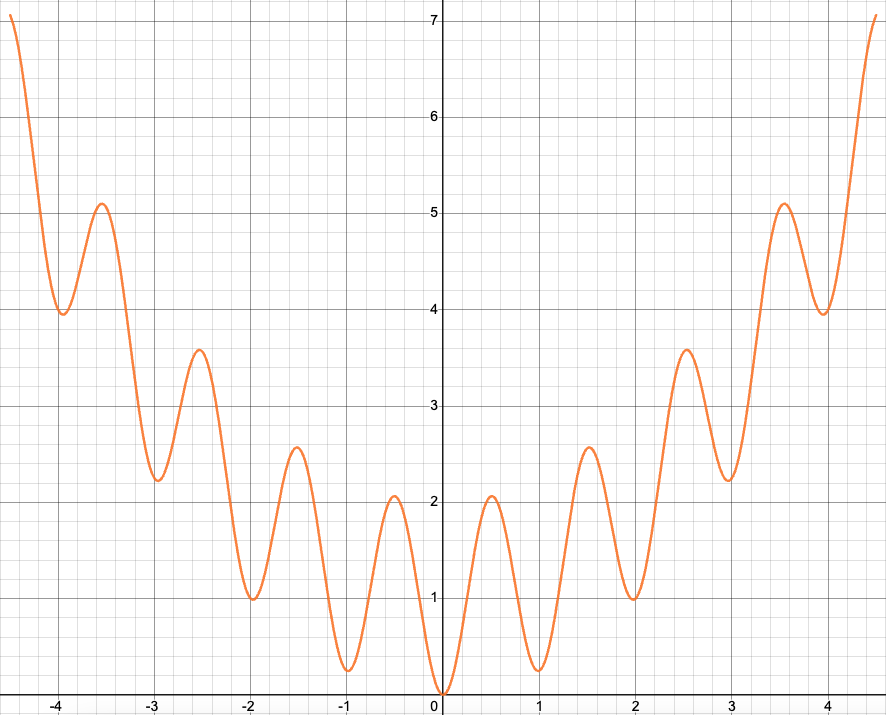
\includegraphics[scale=.25]{474-2-1.png}

%------------------------------------------------------------------------------------------

%---------------------------------------- 1B DONE -----------------------------------------
        
        \item Find an initial point $x_0$ where gradient descent could end up converging to a local minimum that is not the global minimum.

        \color{blue}\textbf{Answer:} $x_0 = 1.5$ \color{black}

%------------------------------------------------------------------------------------------

%---------------------------------------- 1C DONE -----------------------------------------
        
        \item Find a subset of $[-4.5, 4.5]$ such that f(x) has a non-unique global minimum.

        \color{blue}\textbf{Answer:} [0.328, 0.688] \color{black}

%------------------------------------------------------------------------------------------

%---------------------------------------- 1D DONE -----------------------------------------
        
        \item Find a subset of $[-4.5, 4.5]$ such that f(x) has a unique global minimum.

        \color{blue}\textbf{Answer:} $[-0.1, 0.1]$\color{black}

%------------------------------------------------------------------------------------------

    \end{enumerate}

%----------------------------------------- 2 DONE -----------------------------------------

    \item Consider the linear regression problem in the previous lectures. Recall the "real estate" data set (see code on Canvas and more details in the slides). Consider the data set as it stands (i.e., incorporating all six $x$ features and the target $y$ being the house price of unit area). Given the candidate function
    \begin{displaymath}
        y = \omega^Tx + b, \omega \in \R^6, b \in \R,
        \tag*{(1-4)}
    \end{displaymath}
    and the cost function defined as RSS (unless noted otherwise), consider the following questions. Note the gradient formulation (if used) is expected to be derived analytically (then implemented in code), but the calculation of gradients can be done numerically in a variety of ways. As a result, your Python code is expected to use only standard Python libraries and \texttt{numpy} only.
    
    \begin{enumerate}[label=(\alph*)]

%---------------------------------------- 2A DONE -----------------------------------------
    
        \item Starting from the initial point at $\omega = \begin{bmatrix} 1 & 1 & 1 & 1 & 1 & 1\end{bmatrix}^T$ and $b = 10$, execute the gradient descent algorithm for 4140 steps at a constant learning rate $\gamma = 0.001$, what is the updated solution (you are extremely likely to need some help from your computer here)?

        \color{blue}\textbf{Answer:} $\omega = \begin{bmatrix} 0.72 & 0.09 & 0.17 & 0.02 & 0.05 & 0.33\end{bmatrix}^T$ and $b = 3.42$ \color{black}

%------------------------------------------------------------------------------------------

%---------------------------------------- 2B DONE -----------------------------------------
        
        \item If you follow the configuration described in the previous question (i.e., same initial point, same learning rate), for a sufficiently large running steps, will Gradient Descent lead you to the same optimal solution you have derived from the regression lecture (in other words, will it converge?)? Why?

        \color{blue}\textbf{Answer:} It will converge, but to a local optima, not a global optima. Therefore, it will not lead you to the same optimal solution.\color{black}

%------------------------------------------------------------------------------------------

%---------------------------------------- 2C DONE -----------------------------------------
        
        \item Starting from the initial point at $\omega = \begin{bmatrix} 1 & 1 & 1 & 1 & 1 & 1\end{bmatrix}^T$ and $b = 10$, execute the stochastic gradient descent algorithm for 4140 steps at a constant learning rate $\gamma = 0.001$ (let's say an invisible magical force is controlling the generation of all randomness on our planet, and your "stochastic" samples end up being the enumeration of the 414 points in the real estate data set following the exact order as it stands in the .csv file, thus to have the 4140 steps, you will have to repeat the enumeration at the same order for 10 times), what is the updated solution? Is your solution better than, the same with, or worse than the solution from 2(a)? Why?

        \color{blue}\textbf{Answer:} $\omega = \begin{bmatrix} 0.59 & 0.04 & 0.9 & 0.01 & 0.03 & 0.25\end{bmatrix}^T$ and $b = 2.41$. Better than, because it converges to a global minimum rather than a global maximum.\color{black}

%------------------------------------------------------------------------------------------

%---------------------------------------- 2D DONE -----------------------------------------
        
        \item Let's consider a cost that is not RSS, but takes the following form:\\
        \begin{displaymath}
            J(X, y;\omega, b) = \sum\limits^n_{i=1} |y_i - \omega^Tx_i - b|.
            \tag*{(1-5)}
        \end{displaymath}

        \begin{enumerate}[label=\roman*.]

%------------------------------------------------------------------------------------------

%---------------------------------------- 2Di DONE ----------------------------------------
        
            \item Is the optimal solution unique? If the optimal solution is not unique, why? If it is unique, is it still the same with the original one derived from the RSS cost?

            \color{blue}\textbf{Answer:} It is not unique because the absolute value property makes it so that it has more than 1 solution. Thus, it is not unique.\color{black}

%------------------------------------------------------------------------------------------

%--------------------------------------- 2Dii DONE ----------------------------------------
        
            \item For sufficiently large running steps with learning rate $\gamma = 0.001$, can you prove the convergence of Gradient Descent using the updated cost function (1-5)? Why?

            \color{blue}\textbf{Answer:} We cannot prove the convergence of Gradient Descent due to the inability to find the gradient of an absolute value function.\color{black}

%------------------------------------------------------------------------------------------

        \end{enumerate}
    \end{enumerate}

%----------------------------------------- 3 DONE -----------------------------------------

    \item A manufacturing company produces a product using different materials. The goal is to minimize the production cost while meeting certain quality constraints. The company uses three materials, A, B, and C, in varying quantities to produce one unit of the product. THe cost per unit of each material is as follows:

        \begin{itemize}
            \item Material A: \$4 per unit
            \item Material B: \$7 per unit
            \item Material C: \$3 per unit
        \end{itemize}

    Additionally, the company must meet the following quality constraints for each unit produced:

        \begin{itemize}
            \item The product must contain at least 20 units of Material A.
            \item The product must contain at least 15 units of Material B.
            \item The product must contain at least 10 units of Material C.
        \end{itemize}

    The company wants to determine the optimal quantities of each material to use in production to minimize the total cost while satisfying the quality constraints.
    
    \begin{enumerate}[label=(\alph*)]

%---------------------------------------- 3A DONE -----------------------------------------
    
        \item Formulate the above problem as an optimization problem.

        \color{red}\textbf{Answer:} Bowen said to ignore this question...\color{black}

%------------------------------------------------------------------------------------------

%---------------------------------------- 3B DONE -----------------------------------------
        
        \item Solve it with Gradient Descent.

        \color{red}\textbf{Answer:} Bowen said to ignore this question...\color{black}

%------------------------------------------------------------------------------------------

    \end{enumerate}
\end{enumerate}

%------------------------------------------------------------------------------------------

%----------------------------------------- 4 DONE -----------------------------------------

\section{A ``Bonus" Question, This is the Last Time (1 pt)}

\noindent From a scale of 1 to 5, how difficult is HW3? 1 is ``I can do it in my sleep". 5 is ``Bowen is ridiculous". 0 is ``I refuse to answer this question". This is for my own reference to improve the quality of future assignments. Thanks!

\noindent \color{blue}\textbf{Answer:} 5. I was so confused for a lot of this assignment and didn't really know how to ask questions to understand it. Also, the python questions are extremely difficult since I've never learned Python and I spent too much time on the other questions to have enough time to actually figure out how to do them.\color{black}

%------------------------------------------------------------------------------------------
    
\end{problem}
\end{document}